
% new fig
\begin{figure}
    \centering
    \begin{subfigure}{.4\textwidth}
        \centering
        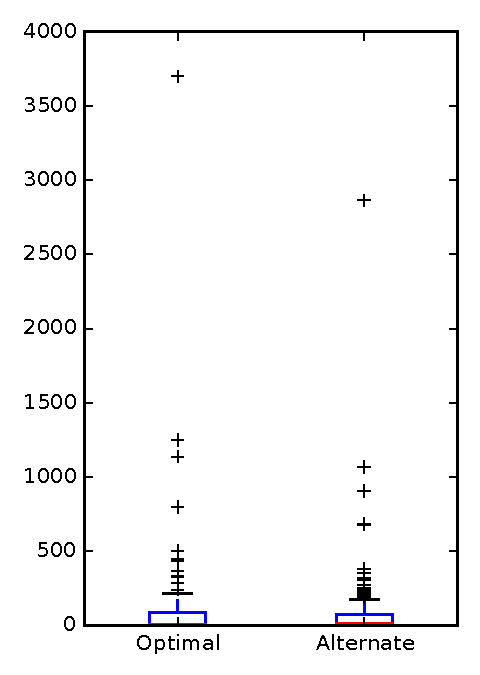
\includegraphics[height=0.4\textheight]{figures/combo/flt_rq1_openjpa}
        \caption{Including outliers}\label{fig:combo:flt:rq1:openjpa_outlier}
    \end{subfigure}%
    \begin{subfigure}{.4\textwidth}
        \centering
        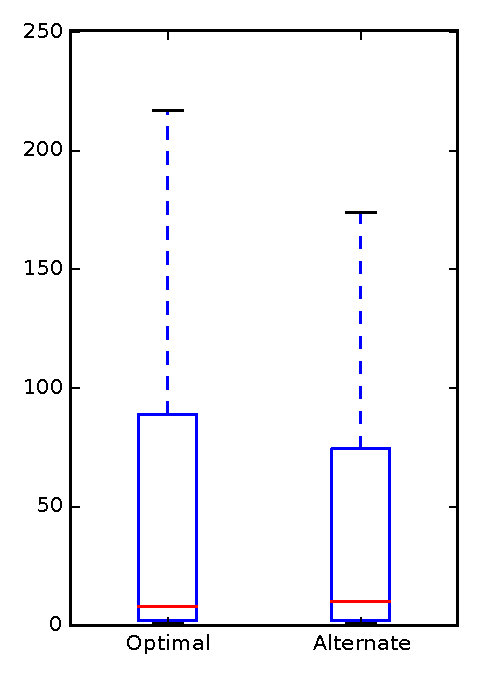
\includegraphics[height=0.4\textheight]{figures/combo/flt_rq1_openjpa_no_outlier}
        \caption{Excluding outliers}\label{fig:combo:flt:rq1:openjpa_no_outlier}
    \end{subfigure}
\caption[Feature Location effectiveness measures of optimal and alternate model configurations for OpenJPA v2.3.0]%
{Feature Location effectiveness measures of optimal ($MRR=0.3089$) and alternate ($MRR=0.2983$) model configurations for OpenJPA v2.3.0}
\label{fig:combo:flt:rq1:openjpa}
\end{figure}
